\section{Clinical applicability}

\begin{frame}[plain,c]
    %\frametitle{A first slide}

    \begin{center}
        \color{DarkBlue}
    \Huge \thesection. \insertsection
    \end{center}

\end{frame}


\begin{frame}{Learnlets - 1~[Ramzi et al. 2021a]}
    % show the generalization figure
    \begin{exampleblock}{Contribution \#4}
        \fullcite{Ramzi2021WaveletsEra}
    \end{exampleblock}
    \begin{figure}
        \centering
        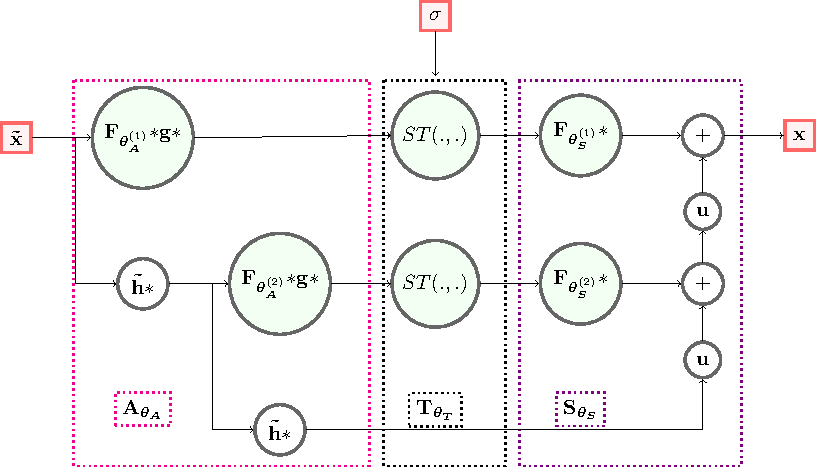
\includegraphics[height=0.53\textheight]{Figures/clinic_applic/learnlets_tikz_reduced.pdf}
    \end{figure}
    \let\thefootnote\relax\footnotetext{
        ST: Soft Thresholding
    }
\end{frame}

\begin{frame}{Learnlets - 2~[Ramzi et al. 2021a]}
    % show the generalization figure
    \begin{figure}[ht]
        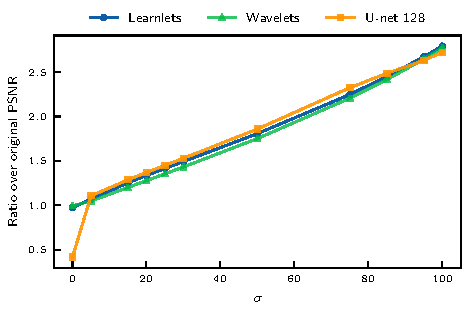
\includegraphics[height=0.78\textheight]{Figures/clinic_applic/model_comparison.pdf}
        \caption{\textbf{Denoising performances.}}
        \end{figure}

    \begin{tikzpicture}[overlay,remember picture,>=stealth,nodes={align=left,inner ysep=1pt},<-]
        \draw[draw=red!47, dashed, visible on=<2>] (3.5cm,2cm) rectangle ++(0.8cm,2.1cm);
        \draw[draw=red!47, dashed, visible on=<2>] (10.7cm,6cm) rectangle ++(1.5cm,1.4cm);
    \end{tikzpicture}
\end{frame}

\begin{frame}{Denoising Score Matching - 1~[Ramzi et al. 2020d]}
    % show the samples
    \begin{exampleblock}{Contribution \#5}
        \fullcite{Ramzi2020_dsm}
    \end{exampleblock}
    Optimal denoiser $\rb^\star$:\footfullcite{Vincent2011,Alain2013}
    \begin{equation*}
        \rb^\star(\tikzmarknode{image}{\highlight{yellow}{$\xb'$}}, \sigma) = \xb' + \sigma^2 \overbrace{\nabla_{\xb} \log \tikzmarknode{prior}{\highlight{blue}{$p_{\sigma^2}$}}(\xb')}^{Score}
    \end{equation*}
    \begin{tikzpicture}[overlay,remember picture,>=stealth,nodes={align=left,inner ysep=1pt},<-]
        % For "prior"
        \path (prior.south) ++ (0,-2.7em) node[anchor=south west,color=blue!87] (exp_prior){
            Convolved prior distribution\\
            $p_{\sigma^2} = p \ast \mathcal{N}(0, \sigma^2)$
        };
        \draw [color=blue!87](prior.south) |- ([xshift=-0.3ex,color=blue]exp_prior.south east);
        % For "image"
        \path (image.north) ++ (0,0.7em) node[anchor=south east,color=amber!87] (exp_image){
            Noisy image
        };
        \draw [color=amber!87](image.north) |- ([xshift=-0.3ex,color=amber]exp_image.south west);
    \end{tikzpicture}
\end{frame}

\begin{frame}{Denoising Score Matching - 2~[Ramzi et al. 2020d]}
    % show the samples
    \begin{figure}
        \centering
        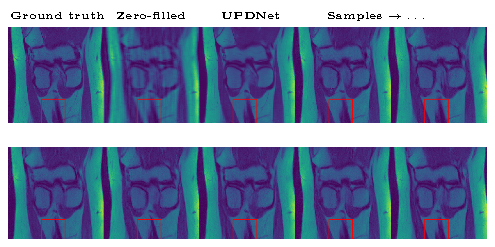
\includegraphics[width=\textwidth]{Figures/clinic_applic/dsm_main.pdf}
    \end{figure}

\end{frame}
